\section {Estudo de Caso}

Visando à validação da solução apresentada na Seção \ref{sec:solucao}, foram consultadas as instituições citadas pelo Acórdão nº 2314/2013 \cite{TCU:2013}. Entre elas, o Instituto do Patrimônio Histórico e Artístico Nacional (IPHAN), autarquia da administração pública federal responsável pela gestão de diversos processos de preservação do patrimônio cultural, permitiu o acesso ao processo, documentos e o código-fonte do SICG, um dos primeiros softwares desenvolvidos sob contrato de terceirização de serviços com a utilização de metodologias ágeis. Essa aplicação foi desenvolvida na linguagem Java com a utilização de \textit{frameworks} como VRaptor e Hibernate, durante 24 \textit{releases} mensais. Possui um total 39.790 linhas de código distribuídas em 914 classes.

\subsection{Protocolo do Estudo de Caso}
Seguindo a metodologia proposta por Wohlin \cite{wohlin2012experimentation}, foi construído um protocolo de estudo de caso, baseado em Brereton \cite{brereton2008using}, quanto aos aspectos gerais e Yin \cite{yin2011applications} com relação as ameaças à validade do estudo. 

O objeto do estudo de caso é o ambiente de \textit{Data Warehousing} (DWing) projetado e implementado conforme apresentado na seção 3. A unidade de análise foi o código fonte do SICG. A partir do objetivo da pesquisa, foram elaborados objetivos específicos do estudo de caso utilizando o \textit{Goal Question Metric} (GQM) \cite{Basili96b}. Nesta abordagem cada objetivo específico originou uma série de questões específicas respondidas com métricas específicas, tal como se mostra na Tabela \ref{tbl:obj}.

\begin{table}[ht]
\centering
\caption{Objetivos Específicos do Estudo de Caso}
\addtolength{\belowcaptionskip}{6pt}
\input{tabelas/objetivos.ltx}
\label{tbl:obj} 
\end{table}
\FloatBarrier


Com relação às ameaças citadas por Yin, a ameça à validade de construção foi mitigada com utilização da abordagem GQM, uma vez que esta estratégia estabelece uma lógica que une as proposições às métricas utilizadas no estudo. A validade interna é obtida quando se consegue observar as relações causais e todos os elementos que as compõem. No presente estudo de caso, pela própria definição de $T_r$, há uma relação diretamente proporcional à $C_e$, e inversamente proporcional à $C_l$, estabelecendo as relações causais. Quanto à validade externa, destaca-se que a utilização de um estudo de caso não é suficiente para generalizar os resultados deles obtidos, sendo necessária a utilização de estudo em múltiplos casos, a fim de aumentar o poder de generalização \cite{yin2011applications}. Com relação à confiabilidade, a partir da documentação da implementação do ambiente de \textit{Data Warehousing} conjuntamente com o protocolo de estudo de caso e as bases de dados das métricas de código-fonte, garante-se a repetição do estudo de caso e, por conseguinte, a confiabilidade.

\subsection{Execução e Resultados do Estudo de Caso}
\label{sec:resultados}
Para analisar os cenários de limpeza de código-fonte, foram extraídas as métricas de cada classe e analisadas conforme a Tabela \ref{tab:cenarios}. Para cada \textit{release}, foram identificados, conforme a Figura \ref{fig:cenarios-release}, os cenários de limpeza de código-fonte. Para se mostrar maior nível de detalhes dos cenários de limpeza de código-fonte, realizou-se uma consulta OLAP de \textit{Drill-Down}, que tem objetivo de expor mais detalhes na visualização dos dados \cite{Kimball2002}, sobre o modelo dimensional do \textit{data warehouse}. 


\begin{figure}[ht!]
\centering
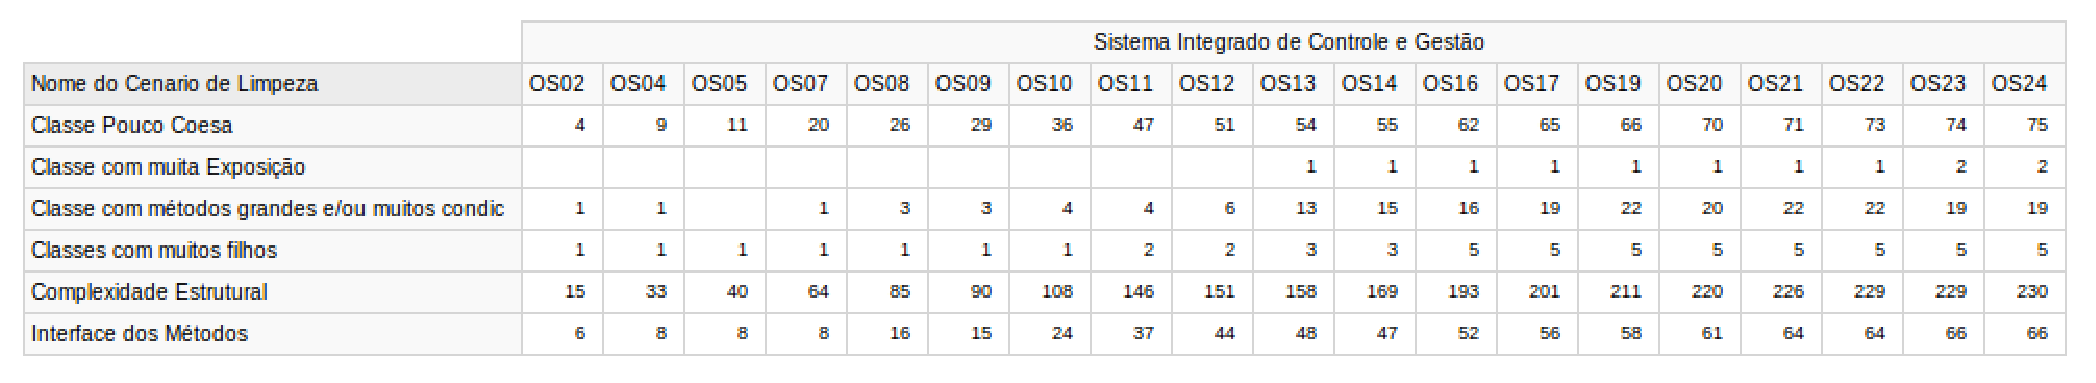
\includegraphics[keepaspectratio=true,scale=0.43]{figuras/total-cenario-tipo.eps}
\caption{Total de Cenários de Limpeza de Código-Fonte identificados por cenário e \textit{Release}}
\label{fig:cenarios-release}
\end{figure}
\FloatBarrier

Conforme é possível observar na figura \ref{fig:cenarios-release}, foram detectados mais cenários de limpeza de código-fonte dos tipos \textbf{Complexidade Estrutural}, \textbf{Classe Pouco Coesa} e \textbf{Interface dos Métodos} respectivamente. Os três Cenários de Limpeza com menor número de incidências foram \textbf{Classe com Muita Exposição}, \textbf{Classe com Muitos Filhos} e \textbf{Classe com Métodos Muito Grande e/ou com muitos condicionais}.

Ao analisarmos os dados conforme apreentado na figura 4-(a) e (b), encontramos uma correlação positiva perfeita entre a quantidade de classes e quantidade de cenários, ou seja, ambas cresceram proporcionalmente na mesma direção, onde r=0,9972. Isso indica que o esforço de refatoração realizado não foi proporcional às necessidades de melhoria do código, nem tampouco direcionado ao tipo de oportunidade de melhoria de maior incidência. Outro sim, é possível inferir que houve pouca atenção da equipe em tomar em boas decisões de projeto(\textit{desing}), em relação a aspectos de modularidade, uma vez que o cenário de complexidade estrutural apresentou uma incidência de 58\% dentro os total de cenários identificados.

\begin{figure}[ht!]
\centering
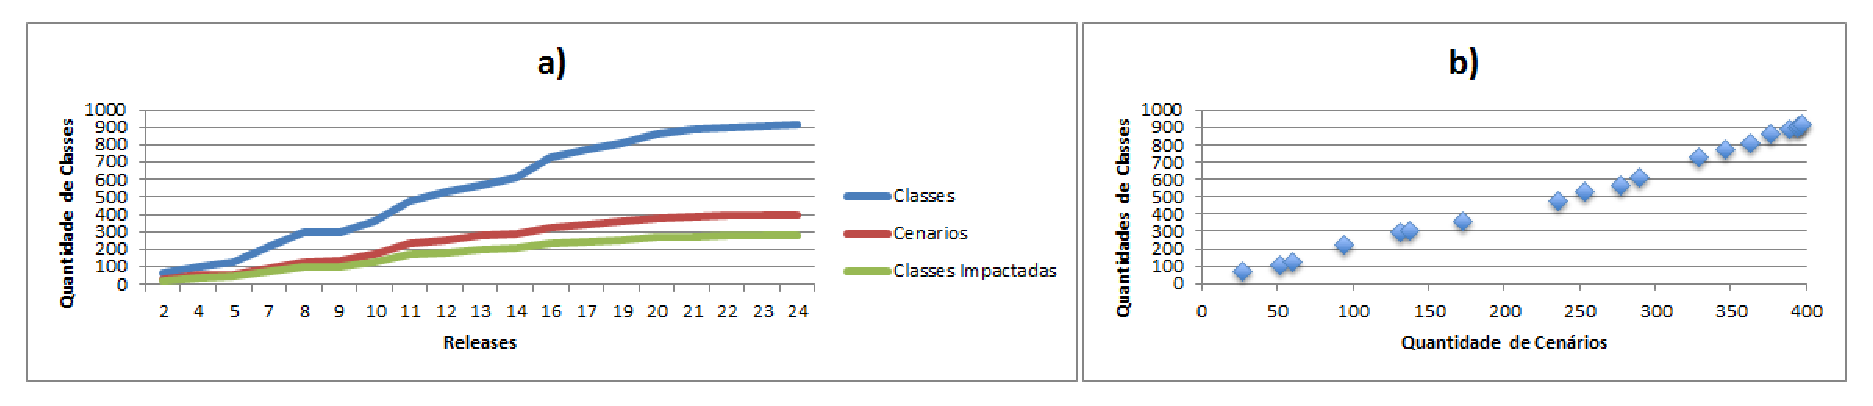
\includegraphics[keepaspectratio=true,scale=0.5]{figuras/classesXcenarios.eps}
\caption{(a) Crescimento de classes e cenários ao longo das Releases - (b) Correlação entre quantidade de classes e quantidade de cenários}
\label{fig:classes-cenarios}
\end{figure}
\FloatBarrier

Considerando que é importante conhecer as classes com maior incidência de problemas com relação limpeza de código-fonte, foram identificadas, como se mostra na Figura \ref{fig:worst-10-cenarios}, as 10 classes que apresentaram a maior quantidade de cenários de limpeza de código-fonte. Para se obter a informação desta consulta foram necessárias uma consulta OLAP de \textit{Drill Down} sobre algumas dimensões e outra de \textit{Slice and Dice}, que tem o objetivo de selecionar os dados, sobre o resultado a consulta de \textit{Drill-Down}.    

\begin{figure}[ht!]
\centering
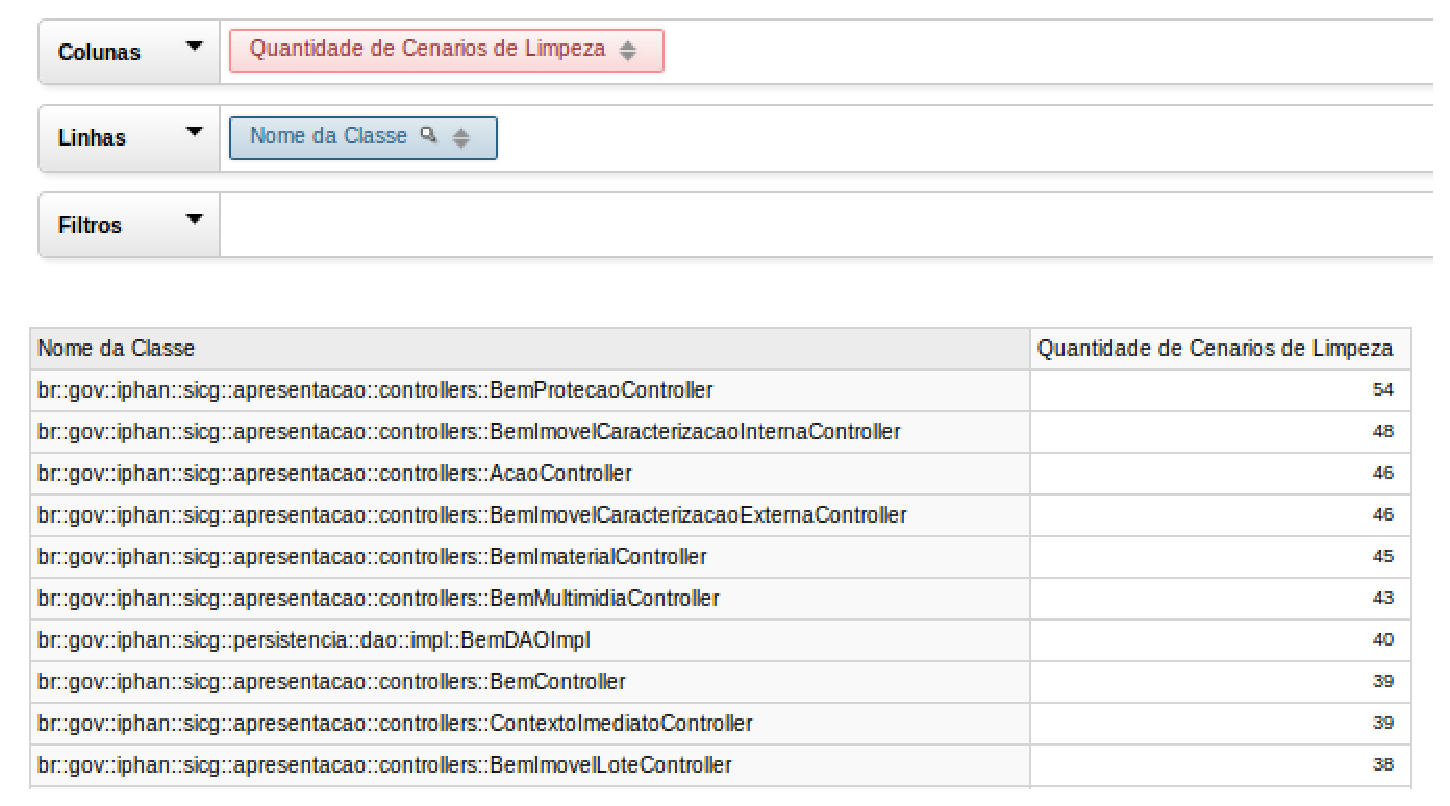
\includegraphics[keepaspectratio=true,scale=0.52]{figuras/10-best.eps}
\caption{As 10 classes com maior número identificado de Cénarios de Limpeza}
\label{fig:worst-10-cenarios}
\end{figure}
\FloatBarrier

Com a quantidade de classes e o total de cenários de limpeza de código-fonte, foi possível calcular a Taxa de Aproveitamento de Oportunidade de Melhoria de Código-Fonte por cada release do software conforme se mostra na Figura \ref{fig:taxa-cenarios}.

\begin{figure}[H]
\centering
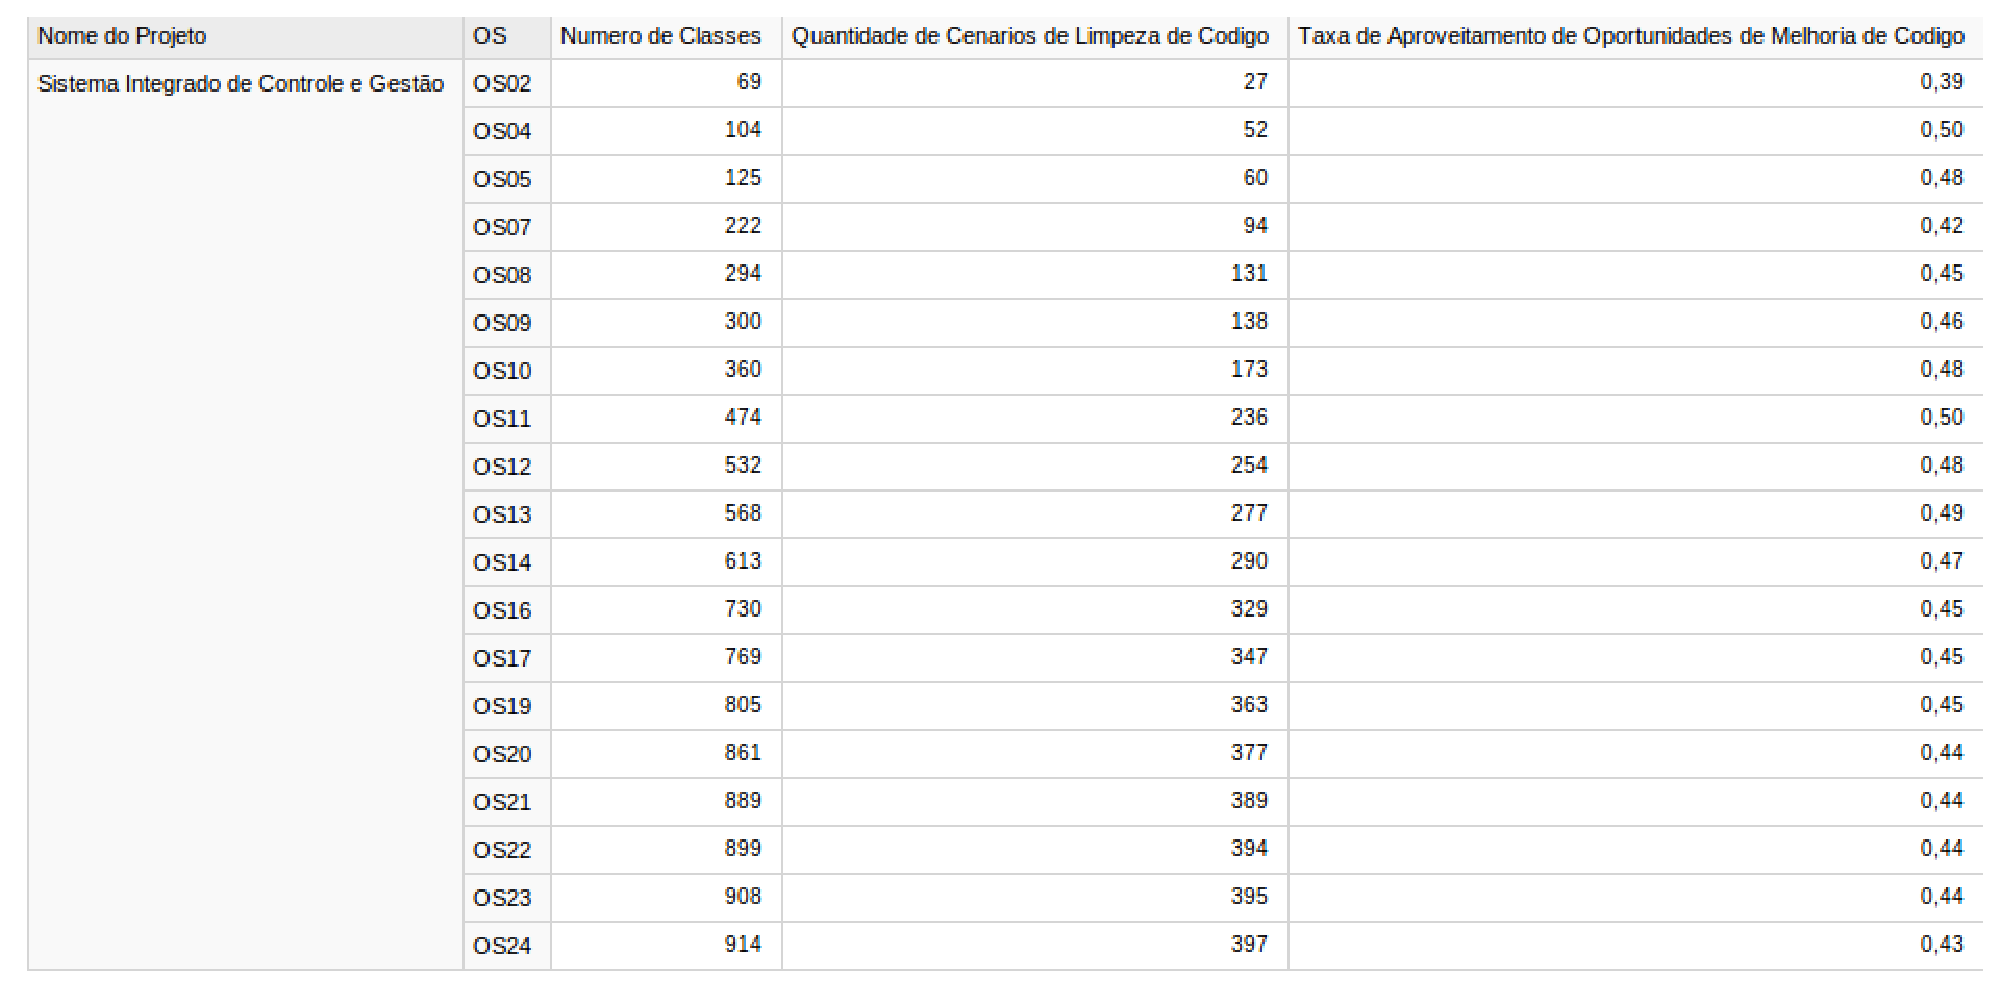
\includegraphics[keepaspectratio=true,scale=0.35]{figuras/taxa-parcial.eps}
\caption{Taxa de Aproveitamento de Oportunidades de Melhoria de Código-Fonte}
\label{fig:taxa-cenarios}
\end{figure}
\FloatBarrier

Ao analisarmos a taxa de oportunidade de melhoria, podemos inferir que: i) apesar do crescimento dos cenários, há uma tendência de estabilidade da taxa a partir da release 16. Isso pode indicar que a equipe adquiriu maturidade sobre o projeto e passou a controlar a qualidade interna, apresentando inclusive, uma suave melhoria.  ii) a melhoria pode não foi significativa em relação às necessidades. Contudo, não houve uma piora desproporcional entre o crescimento do tamanho do código-fonte e dos cenários de oportunidade de limpeza.

A principal dificuldade encontrada com o uso do ambiente de DWing foi o esforço necessário para a construção camada de ETL, amplamente relatado na literatura de referência desta área. Cabe registrar que a definição do esquema do DW pode impactar diretamente as transformações já construídas na camada de ETL. Ou seja, toda vez que realizamos alguma alteração no esquema, tivemos que alterar as transformações previamente construídas na camada de ETL.
Por outro lado, nos beneficiamos da facilidade de automação, flexibilidade para consultas e visualização, disponíveis no DWing.


